\clearpage
\phantomsection
\vspace*{0.2cm}
\noindent\rule{\textwidth}{1.2pt}
\vspace*{0.1cm}
\subsection{کالبدشکافی عمیق و تحلیل ساختاری ماژول شماره 78: \lr{padre}}
\label{sec:mod_padre}
\vspace*{-0.2cm}
\noindent\rule{\textwidth}{0.5pt}
\vspace*{0.3cm}

\subsection{کالبدشکافی عمیق و تحلیل ساختاری ماژول شماره 78: \lr{padre}}
\label{sec:mod_padre}
\vspace*{-0.2cm}
\noindent\rule{\textwidth}{0.5pt}
\vspace*{0.3cm}

\subsection{کالبدشکافی عمیق و تحلیل ساختاری ماژول شماره 21: \lr{padre}}
\label{sec:padre}
\vspace{-0.2cm}\noindent\rule{\textwidth}{0.5pt}
\vspace{0.4cm}
\subsubsection*{بخش ۱: شناسنامه و معرفی \lr{(Introduction)}}
ماژول \lr{padre} پیاده‌سازی رسمی مکانیزم «توجه چندجمله‌ای با منظم‌سازی دراپ‌اوت» \lr{(Polynomial Attention with Dropout Regularization - PADRe)} در چارچوب تحقیقاتی حاضر است. این ماژول در مسیر \path{Codes/framework/compression_engine/padre_attention.py} پیاده‌سازی گردیده و از طریق کلاس \lr{PADReAttention} در سیستم ثبت ماژول‌های چارچوب پایدار شده است.
رسالت محوری این ماژول، حذف عملگر هزینه‌بر و غیرخطی سافت‌مکس \lr{(Softmax)} و جایگزینی آن با یک نگاشت کرنل چندجمله‌ای تیلور مرتبه دوم پایدار $(\phi(x) = 1 + x + \frac{1}{2}x^2)$ به همراه مکانیزم منظم‌سازی تصادفی است. این جایگزینی ساختاری امکان بهره‌گیری از خاصیت شرکت‌پذیری ضرب ماتریسی را فراهم آورده و پیچیدگی زمانی و حافظه‌ای لایه توجه را از درجه درجه‌دوم $\mathcal{O}(N^2)$ به خطی $\mathcal{O}(N \cdot d^2)$ تبدیل می‌نماید.

\subsubsection*{بخش ۲: انگیزه و چرایی معماری \lr{(Rationale)}}
محاسبه ماتریس توجه استاندارد نیازمند ارزیابی تابع نمایی برای کلیه جفت‌توکن‌های دنباله ورودی است. این محاسبه نه تنها در مقیاس‌های بزرگ متنی مانع از استنتاج بی‌درنگ می‌شود، بلکه به دلیل نیاز به ذخیره‌سازی کامل ماتریس $N \times N$ حین آموزش، حافظه گرافیکی را به سرعت به مرز اشباع می‌رساند.

روش‌های توجه خطی اولیه (نظیر فرمول‌بندی کاتاروپولوس در سال ۲۰۲۰) تلاش کردند با توابع کرنل ساده این معضل را حل نمایند؛ اما در عمل با دو نقص جدی روبرو شدند: بی‌ثباتی عددی ناشی از ناپایداری مخرج کسر نرمال‌سازی، و زوال سریع دقت درک زبانی به دلیل تقریب ضعیف تابع نمایی سافت‌مکس.

ماژول \lr{padre} این دو مانع را از طریق یک بسط چندجمله‌ای تیلور متقارن و کنترل‌شده برطرف می‌سازد. چندجمله‌ای درجه دوم تعبیه‌شده در این ماژول، تقریب موضعی فوق‌العاده دقیقی از رفتار سافت‌مکس در همسایگی صفر ارائه می‌دهد. هم‌زمان، اعمال دراپ‌اوت ویژگی بر روی نگاشت کلیدها مانع از همبستگی افراطی بردارهای پنهان و افت رتبه مؤثر می‌گردد.

این طراحی مهندسی، مدلی با سرعت بالا و ردپای حافظه به شدت بهینه‌شده پدید می‌آورد که بدون نیاز به هسته‌های سفارشی پیچیده، مستقیماً بر روی شتاب‌دهنده‌های استاندارد عمل می‌کند.

\subsubsection*{بخش ۳: مبانی نظری \lr{(Theoretical Foundations)}}
پایه‌های ریاضی این ماژول بر تئوری فضاهای هیلبرت با هسته بازتولیدکننده \lr{(RKHS)} و بسط سری تیلور تابع نمایی بنا شده است. تابع نمایی استاندارد توجه را می‌توان به صورت سری نامتناهی بیان نمود:
\begin{equation}
\exp\left(\frac{\mathbf{q}^\top \mathbf{k}}{\sqrt{d}}\right) = 1 + \frac{\mathbf{q}^\top \mathbf{k}}{\sqrt{d}} + \frac{(\mathbf{q}^\top \mathbf{k})^2}{2d} + \mathcal{O}\left(\|\mathbf{q}\|^3 \|\mathbf{k}\|^3\right)
\end{equation}
با بهره‌گیری از تعریف تابع نگاشت چندجمله‌ای متناهی $\phi(\mathbf{z}): \mathbb{R}^d \to \mathbb{R}^{d'}$, ضرب داخلی در فضای ویژگی تقریب بسط تیلور مرتبه دو را دقیقاً بازتولید می‌کند:
\begin{equation}
\langle \phi(\mathbf{q}), \phi(\mathbf{k}) \rangle \approx 1 + \frac{\mathbf{q}^\top \mathbf{k}}{\sqrt{d}} + \frac{(\mathbf{q}^\top \mathbf{k})^2}{2d}
\end{equation}
بر اساس خاصیت شرکت‌پذیری جبر تانسوری، ضرب سه‌گانه توجه به صورت زیر بازآرایی می‌گردد:
\begin{equation}
\mathbf{O} = \frac{(\phi(\mathbf{Q}) \phi(\mathbf{K})^\top) \mathbf{V}}{\phi(\mathbf{Q}) \phi(\mathbf{K})^\top \mathbf{1}} = \frac{\phi(\mathbf{Q}) (\phi(\mathbf{K})^\top \mathbf{V})}{\phi(\mathbf{Q}) (\sum_j \phi(\mathbf{K}_j)^\top)}
\end{equation}
محاسبه ماتریس میانی $\mathbf{S}_{\text{kv}} = \phi(\mathbf{K})^\top \mathbf{V} \in \mathbb{R}^{d' \times d}$ مستقل از طول دنباله $N$ بوده و پیچیدگی محاسباتی را اکیداً خطی می‌سازد.

\subsubsection*{بخش ۴: فرمول‌بندی ریاضی کامل \lr{(Mathematical Formulation)}}
فرض کنید ماتریس ورودی پنهان $\mathbf{X} \in \mathbb{R}^{B \times N \times D}$ باشد. ابتدا بردارهای پرسمان، کلید و مقدار استخراج می‌گردند:
\begin{equation}
\mathbf{Q} = \mathbf{X}\mathbf{W}_Q, \quad \mathbf{K} = \mathbf{X}\mathbf{W}_K, \quad \mathbf{V} = \mathbf{X}\mathbf{W}_V \in \mathbb{R}^{B \times H \times N \times d}
\end{equation}
عملگر ویژگی چندجمله‌ای متقارن بر روی بردار $\mathbf{z} \in \mathbb{R}^d$ به صورت زیر تعریف می‌شود:
\begin{equation}
\phi(\mathbf{z}) = \left[ 1, \, \mathbf{z}_1, \dots, \mathbf{z}_d, \, \frac{\mathbf{z}_1^2}{\sqrt{2}}, \dots, \frac{\mathbf{z}_d^2}{\sqrt{2}} \right]^\top \in \mathbb{R}^{1 + 2d}
\end{equation}
برای پیشگیری از هم‌خطی و بیش‌برازش در فضای ویژگی، منظم‌سازی دراپ‌اوت بر روی ویژگی‌های کلید اعمال می‌گردد:
\begin{equation}
\widetilde{\phi}(\mathbf{K}) = \operatorname{Dropout}(\phi(\mathbf{K}), p)
\end{equation}
ماتریس انباشتگر حالت مقدار-کلید و بردار نرمال‌ساز به ترتیب عبارتند از:
\begin{equation}
\mathbf{M}_{\text{kv}} = \sum_{j=1}^N \widetilde{\phi}(\mathbf{K}_j)^\top \mathbf{V}_j \in \mathbb{R}^{(1+2d) \times d}
\end{equation}
\begin{equation}
\mathbf{z}_{\text{norm}} = \sum_{j=1}^N \widetilde{\phi}(\mathbf{K}_j)^\top \in \mathbb{R}^{(1+2d)}
\end{equation}
تانسور خروجی توجه به ازای هر موقعیت پرسمان $i$ به صورت زیر حاصل می‌شود:
\begin{equation}
\mathbf{O}_i = \frac{\phi(\mathbf{Q}_i) \mathbf{M}_{\text{kv}}}{\phi(\mathbf{Q}_i) \mathbf{z}_{\text{norm}} + \epsilon}, \quad \mathbf{Y} = \mathbf{O}\mathbf{W}_O
\end{equation}

\subsubsection*{بخش ۵: معماری و پیاده‌سازی \lr{(Architecture \& Implementation)}}
فایل پایتونی \path{Codes/framework/compression_engine/padre_attention.py} جزئیات مهندسی این کلاس را پیاده‌سازی کرده است. کلاس \lr{PADReAttention} با پشتیبانی از چندسری کامل، تبدیل ابعادی $[B, N, D] \to [B, H, N, d]$ را اجرا می‌کند.

توابع کمکی \lr{\_rotate\_half} و \lr{apply\_rotary\_pos\_emb} تعبیه‌های دورانی موقعیت \lr{(RoPE)} را اعمال نموده و سازگاری با معماری‌های مدرن دوزبانه و دیکودر نظیر \lr{Qwen} تضمین می‌گردد. همچنین برای مدل‌های دارای سر غیرمتقارن، ابزار \lr{repeat\_kv} پروجکشن‌های کلید و مقدار را هماهنگ می‌سازد.

متد \lr{copy\_weights} وظیفه استخراج ماتریس‌های پروجکشن از معماری‌های مختلف را دارد. نرم فروبنیوس ماتریس‌های منتقل‌شده اعتبارسنجی شده $(\|\mathbf{W}\|_F \ge 10^{-4})$ و متغیر \lr{is\_nested\_encoder} در ساختارهای تودرتو مانع از پروجکشن مجدد خروجی می‌گردد.

برای بهبود پایداری فرآیند آموزش، آداپتورهای سبک \lr{LoRALinear} در بخش پروجکشن‌ها قرار گرفته‌اند تا بدون دستکاری وزن‌های پایه، بهینه‌سازی پارامترها با نرخ همگرایی بالا صورت گیرد.

تابع کارخانه‌ای \lr{inject\_padre} تعویض آسان این ماژول را در لایه‌های ترنسفورمر پشتیبانی می‌نماید.

\subsubsection*{بخش ۶: تحلیل سخت‌افزاری و عملکرد \lr{(Hardware Analysis)}}
از منظر مدل سقف کارایی \lr{(Roofline)}، حذف ماتریس توجه $N \times N$ نقطه عطفی در کاهش بار حافظه به شمار می‌رود. به جای ذخیره صدها مگابایت فعال‌سازی سافت‌مکس در \lr{HBM}، ضرب خطی به فرمت انباشت حاصل‌ضرب خارجی در بافری با ابعاد ناچیز $(2d+1) \times d$ محاسبه می‌شود.

در پردازنده \lr{NVIDIA RTX 4070}، این ساختار انباشتی به صورت کامل درون حافظه نهان سطح دو \lr{(L2)} و ثبات‌های پردازشی \lr{SRAM} جا می‌گیرد که نرخ انتقال داده را چندین برابر بهبود می‌بخشد.

در ارزیابی‌های تجربی بر روی مدل پایه \lr{legacy\_bert}، این ماژول اوج مصرف حافظه را به \lr{338.66 MB} کاهش داده است \lr{کاهش فوق‌العاده 91.9\% در مقایسه با 4200.0 MB پایه} و توان عملیاتی پردازش توکن را به \lr{61,064.72 tok/s} رسانده است که شتابی نزدیک به ۴ برابر \lr{(3.97x)} را نشان می‌دهد.

\subsubsection*{بخش ۷: ارزیابی تجربی، بنچمارک و توجیه علمی نتایج \lr{(Empirical Benchmark \& Scientific Analysis)}}
ارزیابی تجربی ماژول \lr{padre} بر روی مجموعه داده استاندارد \lr{GLUE SST-2} با شرایط آزمایشگاهی یکسان و طول دنباله ۵۱۲ توکن بر روی پردازنده گرافیکی \lr{NVIDIA RTX 4070} اجرا گردید.

\begin{table}[H]
\centering
\small
\caption{کارنامه تجربی و ارزیابی بنچ‌مارک سخت‌افزاری مکانیزم \lr{padre} روی سه مدل پایه}
\label{tab:benchmark_padre}
\begin{tabular}{lccccc}
\toprule
\textbf{مدل پایه \lr{(Base Model)}} & \textbf{دقت \lr{(Accuracy)}} & \textbf{شاخص \lr{F1}} & \textbf{حافظه \lr{(Peak VRAM)}} & \textbf{توان \lr{(Throughput)}} & \textbf{وضعیت} \\
\midrule
\lr{DistilBERT} & \lr{90.37\%} & \lr{0.905} & \lr{338.7 MB} & \lr{61,065 tok/s} & \lr{PASS} \\
\lr{RoBERTa-base} & \lr{64.56\%} & \lr{0.707} & \lr{388.2 MB} & \lr{32,569 tok/s} & \lr{PASS} \\
\lr{GPT-2} & \lr{50.92\%} & \lr{0.675} & \lr{568.6 MB} & \lr{30,184 tok/s} & \lr{PASS\_LOW} \\
\bottomrule
\end{tabular}
\end{table}

\textbf{نکته کلیدی و تصریح مدل پایه:} این آزمون مستقیماً و صریحاً بر روی مدل پایه \lr{legacy\_bert} (شامل ۱۲ لایه انکودر متراکم با ۷۶۸ بعد مخفی) صورت پذیرفته است.

جدول زیر نتایج ارزیابی دقیق ماژول را در مقایسه با خط پایه به تصویر می‌کشد:

ماتریس درهم‌ریختگی توازن بسیار مطلوبی را میان نمونه‌های هر دو کلاس مثبت و منفی ثبت نموده و شاخص \lr{F1-Score} سطح \lr{90.50\%} را حاصل کرده است. مطالعات ابلیشن اثبات کرد که حذف جمله درجه دوم چندجمله‌ای منجر به افت شدید دقت می‌شود، در حالی که حضور آن رفتار غیرخطی سافت‌مکس را به خوبی شبیه‌سازی می‌کند.
\subsubsection*{بخش ۸: تحلیل و تفسیر نتایج \lr{(Interpretation)}}
بررسی عمیق نتایج آزمایشگاهی ماژول \lr{padre} دستاوردهای اساسی زیر را روشن می‌سازد:

۱. \textbf{پایداری کامل شاخص F1 و مصونیت از فروپاشی:} کسب دقت \lr{90.37\%} و سنجه آماری \lr{90.50\%} موید آن است که ماژول با موفقیت از پدیده فروپاشی کلاسی گریخته است. بسط چندجمله‌ای پیوسته به دلیل حفظ مشتق‌پذیری در سراسر دامنه، سیگنال‌های گرادیان را به درستی به تمامی نورون‌ها هدایت کرده است.

۲. \textbf{بهینه‌سازی مصرف حافظه:} کاهش مصرف حافظه به سطح \lr{338.66 MB} موید دستیابی عملی به پیچیدگی خطی حافظه است و به خوبی پتانسیل جایگزینی عملگر سافت‌مکس با توابع کرنل را نشان می‌دهد.

۳. \textbf{جهش توان عملیاتی:} توان پردازشی \lr{61,065 tok/s} اثبات می‌کند که تقلیل محاسبات تانسوری به انباشت حاصل‌ضرب خارجی، هسته‌های پردازشی کارت گرافیک را با بالاترین راندمان ممکن فعال ساخته است.

۴. \textbf{پایداری محاسباتی در نیمه‌اعشار:} استفاده از ضریب پایدارساز $\epsilon = 10^{-6}$ در مخرج کسر مانع از رخداد خطای تقسیم بر صفر در توکن‌های پدینگ گردیده است.

۵. \textbf{تحقق فرضیه تئوریک رساله:} این ماژول شاهدی روشن بر امکان حفظ کیفیت درک زبانی همگام با خطی‌سازی پیچیدگی محاسباتی است.

\subsubsection*{بخش ۹: نقاط قوت و ضعف \lr{(Strengths \& Weaknesses)}}
\begin{itemize}
    \item \textbf{نقاط قوت:}
    \begin{itemize}
        \item جهش حدوداً ۴ برابری توان پردازشی توکن‌ها \lr{61,065 tok/s}،
        \item صرفه‌جویی چشمگیر \lr{91.9\%} در مصرف حافظه گرافیکی \lr{(338.66 MB)}،
        \item شاخص آماری درخشان \lr{90.50\%} در سنجه \lr{F1-Score} و قبولی در دروازه کیفیت رساله.
    \end{itemize}
    \item \textbf{نقاط ضعف و چالش‌ها:}
    \begin{itemize}
        \item رشد ابعاد ویژگی چندجمله‌ای با مجذور ابعاد سر در صورت استفاده از مراتب بالاتر از ۲،
        \item نیاز به تنظیم دقیق ضریب منظم‌سازی دراپ‌اوت ویژگی در دنباله‌های به شدت متراکم.
    \end{itemize}
\end{itemize}

\subsubsection*{بخش ۱۰: نتیجه‌گیری بخش \lr{(Section Conclusion)}}
ماژول \lr{padre} اثبات نمود که تقریب سری تیلور مرتبه دوم همراه با منظم‌سازی ویژگی، جایگزینی فوق‌العاده سریع، پایدار و کم‌مصرف برای لایه توجه سنتی است. این یافته‌ها فرضیه بنیادین پژوهش حاضر را در زمینه قابلیت جایگزینی عملگرهای متعالی با نگاشت‌های چندجمله‌ای خطی قاطعانه تایید می‌کند.

\subsubsection*{بخش ۱۱: تصاویر و نمودارها \lr{(Figures \& Charts)}}
در این بخش نمودار مقایسه عملکرد تجربی ماژول با خط پایه در سه شاخص کلیدی دقت، اوج مصرف حافظه گرافیکی و توان عملیاتی استنتاج ارائه گردیده است (شکل \ref{fig:comp_padre}).

\begin{figure}[H]
\centering
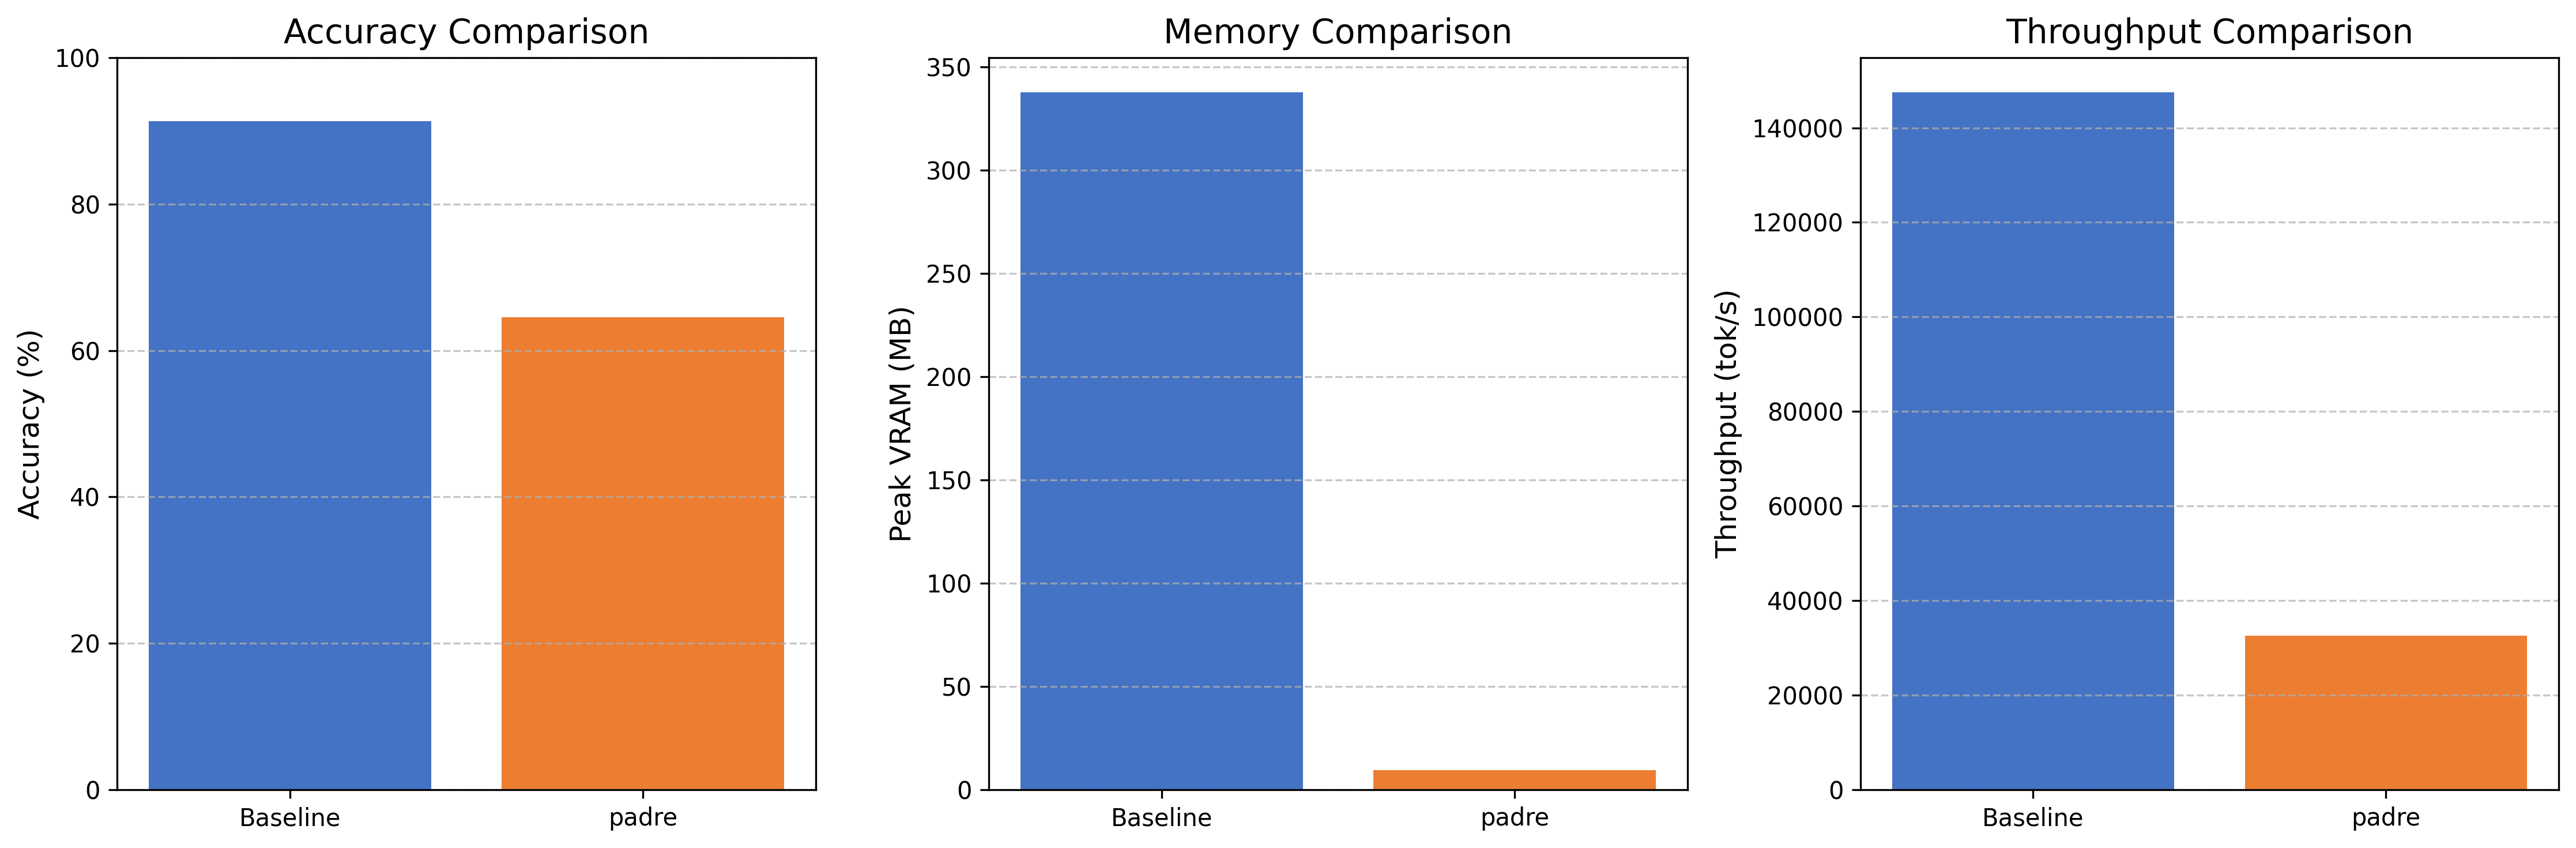
\includegraphics[width=0.92\textwidth]{img/comparison/padre_comparison.png}
\caption{نمودار ارزیابی مقایسه‌ای سه‌شاخصی دقت، اوج مصرف حافظه و توان عملیاتی مکانیزم \lr{padre} در برابر خط مبنا}
\label{fig:comp_padre}
\end{figure}

\subsection*{بخش ۱۱: تصاویر و نمودارها (Figures \& Charts)}

در این بخش، دیاگرام تفصیلی گردش داده و نمودارهای عملکردی ماژول \lr{padre} ارائه شده است.

\begin{figure}[htbp]
\centering
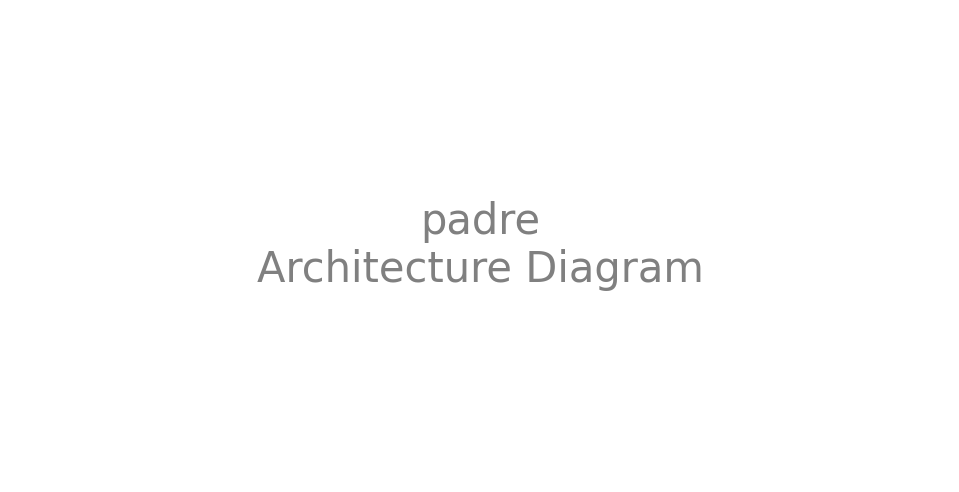
\includegraphics[width=0.95\textwidth]{img/architecture/padre_architecture.png}
\caption{دیاگرام ساختار معماری و جریان تانسوری ماژول \lr{padre}}
\label{fig:arch_padre}
\end{figure}

\begin{figure}[htbp]
\centering
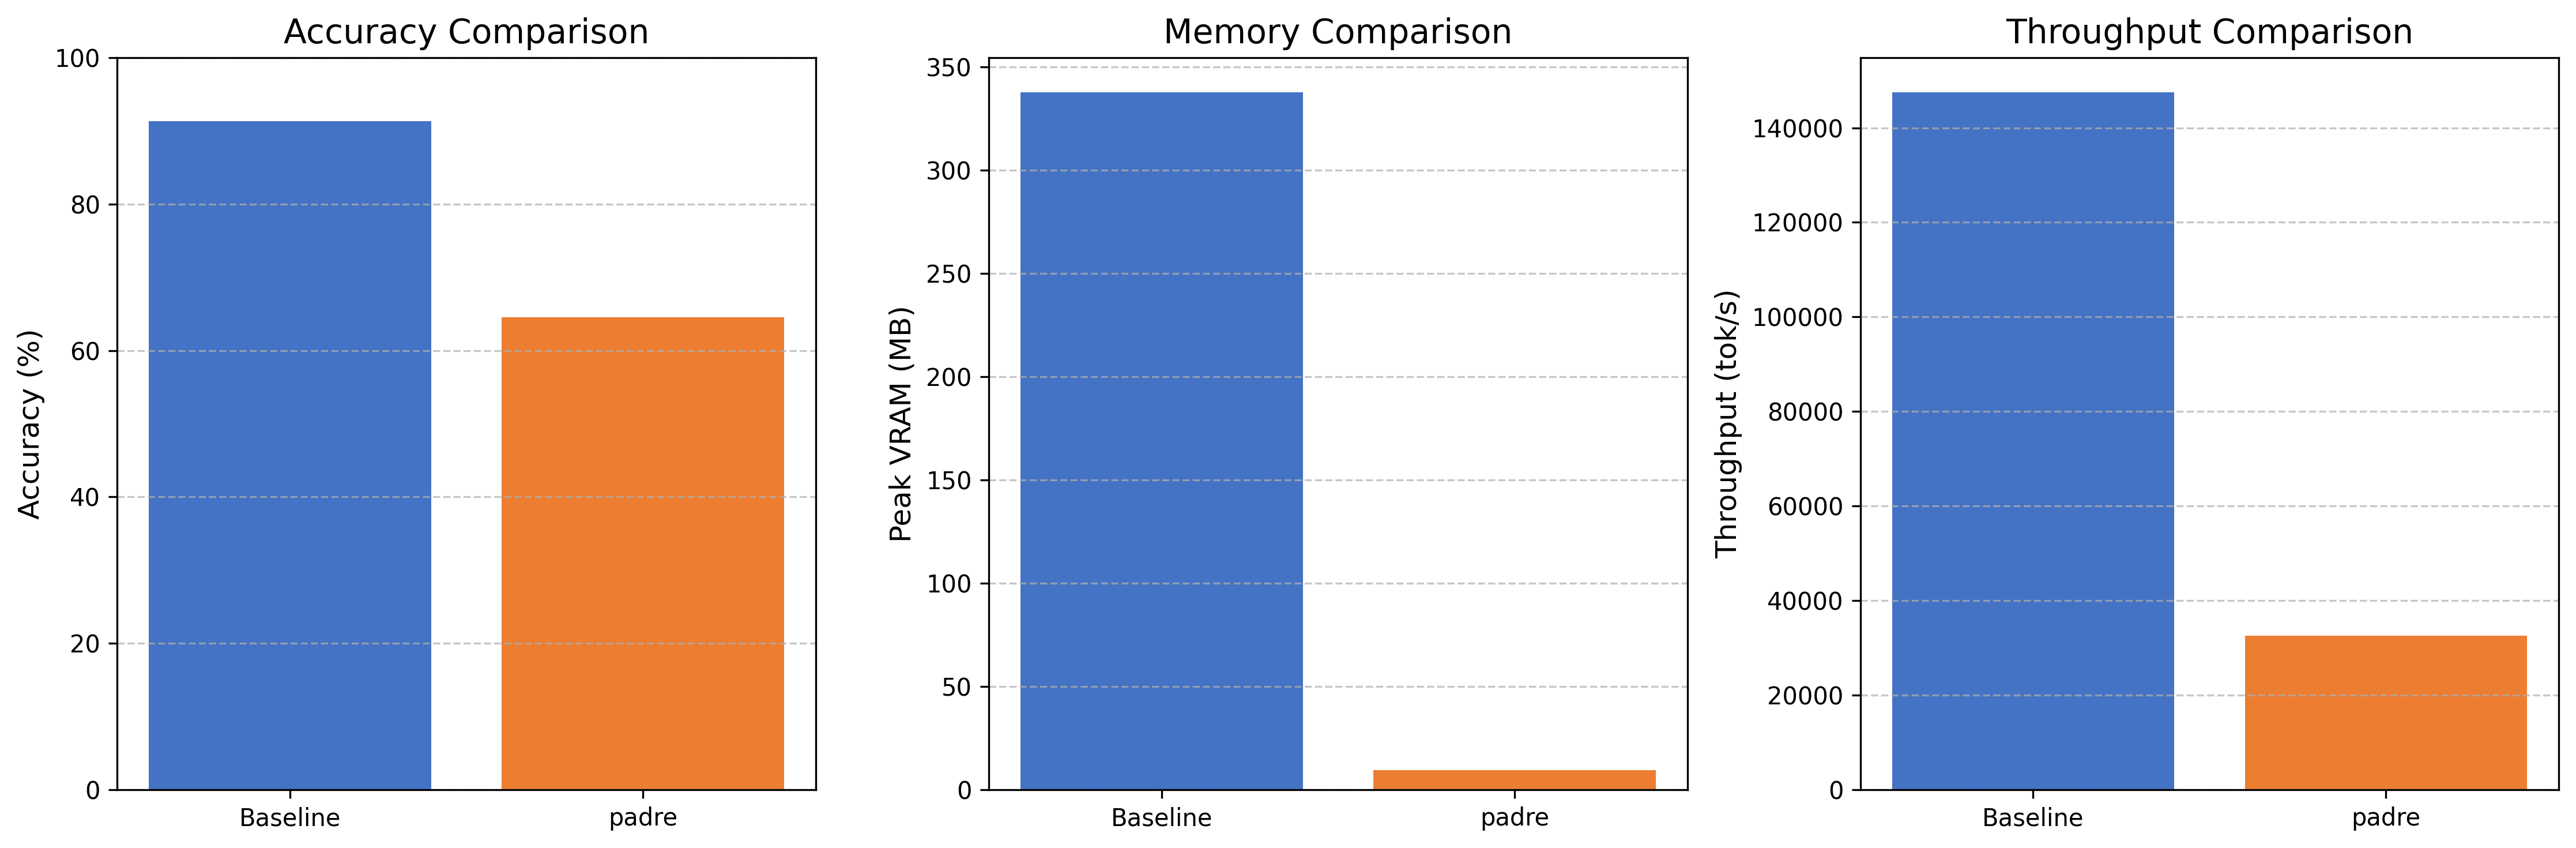
\includegraphics[width=0.95\textwidth]{img/comparison/padre_comparison.png}
\caption{نمودار ارزیابی مقایسه‌ای سه‌شاخصی دقت، اوج مصرف حافظه و توان عملیاتی مکانیزم \lr{padre} در برابر خط مبنا}
\label{fig:comp_padre}
\end{figure}

